
\documentclass[oneside,12pt]{article}
\usepackage[doublespacing]{setspace}
\usepackage[nomarkers,tablesonly]{endfloat}
\usepackage[utf8]{inputenc}
\usepackage{times}
\usepackage{graphicx}
\graphicspath{{images/}}
\usepackage[a4paper, width = 150mm, top = 25mm, bottom = 25mm]{geometry}
\usepackage{fancyhdr}
\pagestyle{fancy}
\fancyhead{}
\fancyhead[R]{The Predictability of Option Intraday Information On Index Returns}
\pagenumbering{arabic}
\usepackage{booktabs}
\renewcommand{\headrulewidth}{0.4pt}
\renewcommand{\footrulewidth}{0.4pt}
\usepackage{caption}
\usepackage{indentfirst}
\usepackage{subcaption}
\usepackage[flushleft]{threeparttable}
\usepackage{hyperref}
\hypersetup{
  colorlinks   = true, %Colours links instead of ugly boxes
  urlcolor     = red, %Colour for external hyperlinks
  linkcolor    = blue, %Colour of internal links
  citecolor   = blue %Colour of citations
}
\usepackage{amsmath}
\usepackage[backend=biber, citestyle = authoryear, bibstyle = authoryear, sorting=nty]{biblatex}
\addbibresource{ref.bib}


\Huge
\title{\textbf{The Predictability of Option Intraday Information On Index Returns}}

\author{I FAN CHIANG}
\date{27 April 2019}



\begin{document}


\maketitle

\begin{abstract}
\centering
The Intraday IVS contains certain imformation about intraday stock return. 

\end{abstract}


\fontsize{13pt}{18pt}\selectfont
\section{Introduction}\label{ch:Introduction}

Probabilistic inference has become a core technology in AI,
largely due to developments in graph-theoretic methods for the 
representation and manipulation of complex probability 
distributions.  Whether in their guise as 
directed graphs (Bayesian networks) or as undirected graphs (Markov 
random fields), \emph{probabilistic graphical models} have a number 
of virtues as representations of uncertainty and as inference engines.  
Graphical models allow a separation between qualitative, structural
aspects of uncertain knowledge and the quantitative, parametric aspects 
of uncertainty...





\fontsize{13pt}{18pt}\selectfont
\section{Hypothesis Development}

\textcite{pan2006information} considers that there is no evidence to prove the informed trading in the index market via performing an regression of the next-day index returns on open-buy put-call ratios. It is a common believe that informed traders tend to hold private information in firm-specific level rather than market-wide level. Therefore, we first exclude the possibility that the predictability of index market may comes from informed-trading. 

In our research, we articulate the intraday CPIV may comes from yesterday trading information and the news beyond market close. Hence, we would like to see in which interval may also contain information toward the contemporaneous index prices and next-day index prices. Apart from prior studies, which possess the best-bid and best-offer of call and put option price within 5 minutes before market close. On top of that, we apply prior approaches to establish CPIV of every interval in a single trading day. We assume that yesterday trading information and news would also reflect in other intervals. In fact, we discuss whether it is appropriate to use the last 5-minutes best bid and best offer to represent the option information in daily frequency. Would it be another chance that other intervals may also be crucial roles in price discovery?  

\begin{description}
\item[Hypothesis 1:] The open and mid intervals may also contain important information toward index returns
\end{description}


\textcite{bergsma2018intraday} spans the results from \textcite{easley1998option} that intraday signed option to stock ratios (O/S) have strong stock return predictability especially in the first 30 minutes of market open. They make a statemtent that the first half hour of trading has predictive power for the remainder of the trading day. In line with this study, we believe CPIV also reflect the market sentiment like O/S. Consequently, we suggest S\&P 500 index option carry information toward the index market, and the information would get incorporated into the index market as time flows. 

\begin{description}
\item[Hypothesis 2:] The first 5-minutes CPIV has predictability during the rest of the trading day
\end{description}






\fontsize{13pt}{18pt}\selectfont
\section{Data and Empirical Methodology}

\subsection{Deviation From Put-Call Parity}
The put-call parity relations derived from \textcite{stoll1969relationship} is a classical option pricing concepts in finance. It characterized the relationship that must exist between European put and call options with the identical underlying asset, expiration and strike prices. The equation must hold for European options given on no-dividends paying underlying in a perfect market. 
\begin{equation}
C-P = S - PV(K)
\end{equation}
Where C and P represent call prices and put prices, and S is Stock price. With same maturity and exercise price K, the arbitrage opportunity would exist if the equation does not hold. The \textcite{black1973pricing} formula satisfies the put-call parity for an assumed value of the volatility parameter $\sigma$, therefore, 
\begin{equation}
C^{BS}(\sigma ) + PV(K) = P^{BS}(\sigma ) + S
\end{equation}
where $C^{BS}(\sigma )$ and $P^{BS}(\sigma )$ indicate Black-Scholes call and put prices, respectively. 
\\
Combine the above equation, we can derive the equation
\begin{equation}
C^{BS}(\sigma ) - C = P^{BS}(\sigma ) - P
\end{equation}
which implies that the implied volatility of call option and put option should be the same if all equation holds. 
\begin{equation}
IV^{call} = IV^{put}
\end{equation}
Of course, the equation may not hold once the option is American-style. However, our primary studies, SPX option, is European style. Therefore, we do not need to consider the dividend payment or early exercise case in our further research. 

Clearly, the larger the implied volatilities, the higher the call (put) options prices claim. Following \textcite{amin2004index}, we refer to the difference between call and put implied volatilities as the call-put implied volatility spreads (CPIV). It is suggested that a positive (negative) CPIV could be viewed as a bullish (bearish) signal regarding the underlying stock. 

The aggregate Intraday CPIV are construced as following steps: 
\begin{enumerate}
\item  We first divided a single day into 14 of 5-minutes intervals. Each interval contains the tick data from 2.5 minutes ahead and behind the clock. For example, the 9 a.m. interval, we collect valid data from 08:47:30 to 09:32:30 to represent this interval. As for open (close) interval, we choose to accumulate the full 5 minutes data behind (ahead)\footnote{We collect the whole transaction data in 5 minutes for trade data. However, the size of quote data is extremely unbalanced in different intervals, we restricted 1000 to 2000 quotes as maximum for call and put in collecting quote data.}

\item Similar to \textcite{xing2010does}, in each interval, we eliminate an option from the sample if its time to expiration is less than 10 days or more than a year, if its open interest is negative, if its moneyness\footnote{Moneyness is defined as the ratio of the strike price to the stock price.} is smaller than 0.9 or more than 1.1. Furthermore, the option quotes must not violate basic no-arbitrage relations.

\item Then, in each time interval, there must be several valid option pairs with identical maturity (T) and exercise price (K). For each option pair, we choose only one pair to be the representative. For quote data, we average the best bid ($\beta ^{\ast }$) and best offer ($\alpha ^{\ast }$) as the chosen call (put) option price. On the contrary, for trade data, we seize the specific transaction data which is closet to the centering time.  

\item After collecting several time interval valid option pairs. we calculated the CPIV by applying, 
 \begin{equation} \label{eq: withoutadj}
CPIV_{t} = IV_{t}^{call} - IV_{t}^{put} = \sum_{j = 1}^{N_{t}}\theta _{j,t}(IV_{j,t}^{call} - IV_{j,t}^{put})
 \end{equation}
 
$CPIV_{t}$ denotes the implied volatility spread on interval $t$; $IV_{j,t}$ describe the B-S implied volatility for $j^{th}$ option pair in time $t$; $\theta_{j,t}$ are the weight for $j^{th}$ option pair in time $t$, there are $N_{t}$ valid pairs of options on interval $t$. 

Follow by \textcite{holowczak2013aggregating}, the aggregation of option information could be adjusted by the level of moneyness and maturity. 
 \begin{equation} \label{eq: withadj}
CPIV_{t} = IV_{t}^{call} - IV_{t}^{put} = \sum_{j = 1}^{N_{t}}w_{j,t}(IV_{j,t}^{call} - IV_{j,t}^{put})
 \end{equation}

The equation is identical except for the weights term. Ceteris paribus. $w_{j,t}$ equals to $exp(-(m_{j}^{2})/2 -(M_{j} - 1)^{2}) * \theta_{j}$ where $m_{j}^{2}$ measures the moneyness and the $M_{j}$ evaluates the maturity of option contract $j$. To be more specific, $m_{j} =  (\frac{K_{j}}{S_{j}} - 1)$ and $K_{j}$ represents the exercise price and $S_{i}$ acts for the underlying price of option $j$; $M_{j} =  max(1, T_{j}*12) $ and $T_{j}$ represents the maturity of option $j$ in month unit. 


\end{enumerate}


\subsection{Data}
In our analysis, the primary quote and trade intraday data for SPX option originates from CBOE MDR. The sample period studied is from January 2007 to December 2017. The options data includes trade date, trade time, expiration date, put-call code, exercise price, maturities, bid price, ask price, underlying price. The daily price of S\& P 500 index is obtained from Bloomberg. The zero-coupon bond (ZCB) rate represent risk-free rate in B-S formula are collected from WRDS with different duration. The size of the sample data is about 1-TB around and the data amount is about 1 billion. After we exclude the tick data fall outside the 14 of 5-minute intervals, it remains about 40 million. Furthermore, we follow the approach from \textcite{ofek2004limited} to exclude the invalid option pairs. Finally, we have 1,692,542 valid volatility spreads for SPX option from January 2007 to December 2017. 

Following the prior studies \textcite{bollerslev2009expected}, several macro-economic variables are suggested to be crucial and informative with regard to future returns. Specifically, we collect data of the default spread (between Moody's BAA and AAA corporate bond spreads), the term spread (between the 10-year T-Bond and 3-month T-bill yields) \footnote{The daily data are collected from the public website of the Federal Reserve Bank of St. Louis.} as control variables in our regression analysis. The set of macro-economics controls used in regressions changes as the measurement window of the expected market returns changes. 

In our study, the amount of intraday CPIV should be 38,668 (14 Intervals multiply 2,762 Days). However, most of the option quote data are short date contract (less than 10 days) in the middle of the month so that we have multiple values that are not able to calculate by our approach. Meanwhile, our research also winsorized the outliers of intraday CPIV on 1\% at the front and end. The amount of final valid interval CPIV of quote data is 27,554, as for trade data is 36,959.


\autoref{table:stats_of_CPIV} presents the descriptive statistics of intraday CPIV. In panel A, we demonstrate the descriptive statistics on CPIV of intervals. The mean (median) CPIV vary from -2.45 \% to -3.65 \% (-3.32 \% to -3.72\%), indicating that, on average, S\&P 500 index put option has about three percent higher implied volatility than index call option during our sample period. In fact, the results are similar to \textcite{atilgan2015implied}, they put forth the observation that on average there are nine percent higher during their sample period. In the index market, the implied volatility to moneyness graph mostly shows a reverse skew, which prior studies \parencite{zhang2008implied} claimed it volatility smirk. Our observations also express this phenomenon. In addition, in panel A, we could tell that the CPIV of open interval (08:30) is completely different from other interval CPIV. The mean of $CPIV_{0830}$ is about 1\% higher than other intervals, and the standard deviation of $CPIV_{0830}$ is 0.4\% higher than others. Furthermore, the amount of positive CPIV is way larger than other intervals. We suggest during the open interval, numerous news and trading information flow in and cause the open-interval CPIV more volatile. Furthermore, the call options are more likely to be relatively expensive than put options in the first interval. We suggest that if investors exposure to good news before the market open, they prefer to reflect on option price in the first 5-minutes.  

In panel B, we test the population mean among the intervals CPIV. 
\begin{equation}
H0: \mu _{i} = \mu _{j}
%H1: \mu _{i} \neq  \mu _{j}
\end{equation}
The p-values of pairs are shown in corresponding rows and columns. From the results, we declare that the population means of $CPIV_{0830}$ are significantly different from other intervals, so does the close interval CPIV. In other words, we claim that the population means of mid-interval CPIV are not significantly different from other mid intervals. The mid intervals may gather similar information. 






%\subsection{Figure}
%\autoref{fig:Network} stock trading volume, and stock returns data are taken from CRSP for the construction of control measures.
%
%\begin{figure}[h]
%\centering
%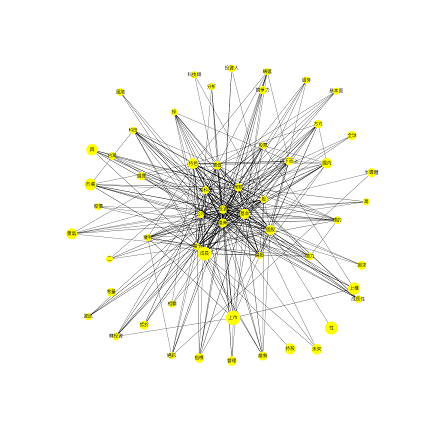
\includegraphics[scale=1.0]{network1}
%\caption{Network ot words}
%\label{fig:Network}
%\end{figure}


\subsection{Empirical Methodology}
Our research divided into two parts. The first part we analysis certain option pair characteristics that cause the deviation of put-call parity. The second part we discuss the relationship between CPIV and index returns in different aspects and frequencies. 

Firstly, we regress CPIV on options characteristics like moneyness, time non-synchronization, maturity, and controlling on intervals effect. The CPIV term and moneyness term are in absolute form because we care about the level of deviations in put-call parity rather than the direction of deviations. 

 \begin{equation}\label{eq:char}
 \footnotesize
\left | CPIV _{i} \right| = \alpha  + \beta _{1}TimeDiff_{i} + \beta _{2}\left |Moneyness_{i} \right | + \beta _{3}Maturity_{i} +  \beta _{j} \sum_{j=1}^{13}IntDummy_{j} +\varepsilon _{i}
 \end{equation}

$TimeDiff_{i}$ represents time non-synchronization in option pair $i$. $Moneyness_{i}$ stands for the level of divergence between the underlying price and the excersie price of option pair $i$. $Maturity_{i}$ symbolizes the maturity date in option pair $i$. As for $IntDummy_{j} $, we control the intervals effect where $j$ denote as each interval, for instance, $IntDummy_{1}$ stands for 09:00. All the t statistics are \citeauthor{newey1986simple} statistics adjusted. 

Secondly, we regress contemporaneous index returns, one day ahead index returns, halh-hours ahead index returns on CPIV and other macroeconomic variables respectively. 
 \begin{equation}  \label{eq:contem}
SPX\_Return_{t} = \alpha + \beta _{1}CPIV_{t} + \beta _{2}DEF_{t} + \beta _{3}TERM_{t} + \varepsilon _{t}
 \end{equation}

In above equation, $SPX\_Return_{t}$ elucidates the SPX index returns in day $t$, where $CPIV_{t}$ could be any interval CPIV within day $t$. $DEF_{t}$ explicates the change in the difference between the yields on BAA- and AAA-rated corporate bonds in day $t$, and $TERM_{t}$ expounds the difference between the yields on the 10-year Treasury bond and one-month Treasury bill in day t. All the t statistics are \citeauthor{newey1986simple} statistics adjusted. 

\begin{equation} \label{eq:1dayahead}
SPX\_Return_{t+1} = \alpha + \beta _{1}CPIV_{t} + \beta _{2}DEF_{t} + \beta _{3}TERM_{t} + \varepsilon _{t}
\end{equation}

In equation (9), the only term we change is $SPX\_Return_{t+1}$. We now regress a day forward returns on dependent variables rather than contemporaneous index returns. 

\begin{equation}
\small
Intra\_Return_{t, k} = \alpha + \beta _{1}CPIV_{t} + \beta _{2}DEF_{t} + \beta _{3}TERM_{t} + \varepsilon _{t},    
\forall k = 1, 2...13-n  
\end{equation}

In this part, we would like to discuss the predictability in intraday index returns, where $Intra\_Return_{t, k}$ means $k$ of half-hour ahead cumulative returns. For example, when we'd like to do research on the intraday returns to $CPIV_{0830}$, $k = 1$ means the cumulative returns from 08:30 to 09:00, and  $k = 2$ means the cumulative returns from 08:30 to 09:30, and so on and so forth. $n$ represents the $n^{th}$ interval CPIV.





\fontsize{13pt}{18pt}\selectfont
\section{Empirical Results}

The main results are based on SPX option quote data. We take both \autoref{eq: withoutadj} (non-adjusted weights) and \autoref{eq: withadj} (adjusted weights) to build intraday CPIV. The results are quite similar, so we only present the results of \autoref{eq: withadj}. The non-adjusted version is upon request.

\subsection{Relationships Between CPIV and Option Characteristic}
Before we explore the relationship between the index returns and CPIV, we need to survey on the option characteristics. From \autoref{eq:char}, We expect the coefficient of time non-synchronization, moneyness. and maturity to be positive. There should be no deviation in put-call parity given that the underlying price is also identical in theroy. In other words, the larger the time gap between the pair option, the larger the divergence may occur and cause higher CPIV in absolute form. Furthermore, the level of moneyness and time to expiration are crucial to CPIV as well. According to \textcite{hentschel2003errors}, implied volatilities from options away from the money are especially sensitive to measurement errors in option prices and uderlying asset price. Therefore, we estimates that with greater level of moneyness and time to maturities, the measurement errors in implied volatilities would increase. 

The results in \autoref{table:regression1} confirm our earlier statements based on regression of CPIV. Column (1) reports the regression of CPIV on time non-synchronization. All the coefficients are highly significant; they imply a positive effect on the deviation of put-call parity. Column (2) of table 5 shows that regression of CPIV on moneyness. The coefficient of moneyness term is also highly significant (0.3833, t-statistic 434.96). Column (3) signifies of CPIV on maturity. The coefficient of maturity term is highly significant (0.0348, t-statistic 296.27) as well. Clearly, the regression results are aligned with previous literature, which indicates the moneyness and maturity have a positive effect on CPIV. Finally, in column (4), we regress CPIV on all option pair characteristics. The outcome is similar to previous regressions. Noticeably, the adjusted $R^{2}$ of moneyness term is almost 34\%, which stands for the most influential factor.  

\subsection{Relationships Between Index Return and CPIV}
In this subsection, we discuss the relationship between CPIV and index returns in different aspects. The Panel A in \autoref{table:regression2} depict the results of contemporaneous index return regressions, while Panel B acts for the results of one-day ahead index return regressions. The header of columns describes the interval of CPIV, and all the variables are in a percentage format. 

In panel A, the CPIV coefficients are all positive and this outcome is aligned with \textcite{cremers2010deviations} which proves the evidence for a significant positive link between implied volatility spread and expected returns. To be more specific, $CPIV_{08:30}$ and $CPIV_{12:00}$ are significant in 1\% and 10\% level respectively. However, other intervals are not significant enough under 10\% level. The result validates our first hypothesis: The open and mid intervals may also contain important information toward index returns. Apart from that, $CPIV_{08:30}$ has the largest coefficient 8.33\footnote{The value is shown in a percentage format.} (t-statistic 17.84), we believe that most trading information and news of previous days get incorporated into the first interval.

In panel B, we test the one day ahead index returns on CPIV and other control variables to see whether the information spillover from the options market to one day ahead index market. Surprisingly, none of them are significant enough and not all of them are positive. According to \textcite{atilgan2015implied}, they assert the volatility skewness of S\&P index option may cause a spillover effect to the index market. We find out the implied volatility spreads have no predictability on aggregate index returns in the one-day horizon. This is slightly different from \textcite{atilgan2015implied} since we choose implied volatility spreads rather than volatility skewness as the measures. The implied volatility spreads absorb all possible option pairs information while volatility skewness only include the information from out-of-money (OTM) put options and at-the-money (ATM) call options. Briefly, the implied volatility spreads may be too noisy in forecasting future index returns.  

On intraday frequency, we also test the predictability on cumulative half hour index returns in different horizons. We only take $CPIV_{08:30}$ and $CPIV_{12:00}$ as independent variables since they are the only variables significant on daily frequency. However, the results are completely not the same way. From \autoref{table:regression4}, the coefficients of $CPIV_{08:30}$ range from 5.63 to 6.57, implying myriad economic significance. The adjusted $R^{2}$ of $CPIV_{08:30}$ range from 50.19\% to 19.17\% as hours decay. The results are consistent with our Hypothesis 2: The first 5-minutes CPIV has predictability on intraday index cumulated returns for the remainder of the same trading day. On the contrary, we did not find predictive power on $CPIV_{12:30}$ for any $k$. In this paragraph, we demonstrate that the first 5-minutes interval keeps considerable information compared to other intervals, and this information would be incorporated into the index market by hours -- not by days. Our empirical results are slightly different from \textcite{cremers2010deviations}, but similar to \textcite{kumar1992behavior}. 
   




%====================================================================
%                        Tables 5
%====================================================================

\begin{table}[h]
\centering
\caption{Regression Results: CPIV and Option Pair Characterisitcs}\label{table:regression1}
\begin{threeparttable}

\medskip

{\scriptsize 
This table shows the regression results of call-put implied volatility (CPIV) on moneyness, time non-synchronization, maturity with intervals fixed effect. The $CPIV$ term and moneyness term are in absolute form because we care about the level of deviations in put-call parity rather than the direction of deviations. $TimeDiff$ represents time non-synchronization. $Moneyness$ stands for the level of divergence between the underlying price and the exercise price. $Maturity$ symbolizes the maturity date. As for Interval F.E., we control the effect of the intervals. All the t statistics in parathesis are Newey-West t statistics adjusted.
}
\medskip
\small
\centering
\begin{tabular}{ccccc}
\toprule
              & (1)        & (2)        & (3)        & (4)        \\ \midrule
Intercept     & 0.05577*** & 0.03087*** & 0.05055*** & 0.03011*** \\
              & (263.91)   & (170.91)   & (229.42)   & (162.73)   \\
TimeDiff      & 0.0000***  &            &            & 0.0000***  \\
              & (89.32)    &            &            & (7.40)     \\
Moneyness     &            & 0.3833***  &            & 0.3710***  \\
              &            & (434.96)   &            & (366.56)   \\
Maturity      &            &            & 0.0348***  & 0.0103***  \\
              &            &            & (296.27)   & (68.17)    \\
Interval F.E. & Yes        & Yes        & Yes        & Yes        \\
No. Obs       & 1692542    & 1692542    & 1692542    & 1692542    \\
Adj. $R^{2}$  & 0.0473     & 0.3368     & 0.0853     & 0.3402     \\
\bottomrule
\end{tabular}

\begin{tablenotes}
%\multicolumn{4}{l}{\footnotesize \textit{Newey-West t} statistics in parentheses} \\
%\multicolumn{4}{l}{\footnotesize * $p < 0.10$, ** $p < 0.05$, *** $p < 0.01$} \\
\item
\item[***]Significant at the 1 percent level.    
\item[**]Significant at the 5 percent level.   
\item[*]Significant at the 10 percent level.
\end{tablenotes}

\end{threeparttable}

\end{table}


%====================================================================
%                        Tables 6, 7
%====================================================================



\begin{table}[h]

\caption{Regression Results: Index Return Predictability on CPIV of Quote Data}\label{table:regression2}
\begin{threeparttable}

\medskip

{\scriptsize 
This table reports from time-series predictive regressions of the daily return of the S\&P 500 index on call-put implied volatility (CPIV), and macroeconomic variables. Panel A presents the summary statistics for contemporaneous index returns regression. Panel B presents summary statistics for one-day ahead index returns regression. $CPIV$ elucidates the interval implied volatility spreads. $DEF$ explicates the change in the difference between the yields on BAA- and AAA-rated corporate bonds. $TERM$ expounds the difference between the yields on the 10-year Treasury bond and one-month Treasury bill. All the t statistics in parathesis are Newey-West t statistics adjusted. All variable values are in a percentage format.  
}
\medskip

\begin{subtable}[t]{\linewidth}

\caption{Panel A: The Contemporaneous Index Return Regression }
\tiny
\begin{tabular}{ccccccccccccccc}
\toprule
	& 08:30   & 09:00   & 09:30   & 10:00   & 10:30   & 11:00   & 11:30   & 12:00   & 12:30   & 13:00   & 13:30   & 14:00   & 14:30   & 15:00   \\ \midrule
Intercept & 0.26*** & 0.15    & 0.17    & 0.16    & 0.14    & 0.21*   & 0.13    & 0.25**  & 0.17    & 0.18    & 0.14    & 0.16    & 0.27**  & 0.31*   \\
      & (2.84)  & (1.47)  & (1.62)  & (1.52)  & (1.32)  & (1.82)  & (1.18)  & (2.07)  & (1.36)  & (1.38)  & (1.02)  & (1.11)  & (1.90)  & (2.04)  \\
CPIV      & 8.33*** & 1.35    & 1.30    & 1.84    & 1.50    & 2.86    & 0.41    & 3.86*   & 2.24    & 2.13    & 1.03    & 2.57    & 4.91    & -0.25   \\
      & (17.84) & (0.85)  & (0.83)  & (1.07)  & (0.85)  & (1.48)  & (0.20)  & (1.83)  & (1.01)  & (1.09)  & (0.51)  & (1.21)  & (1.91)  & (-0.09) \\
DEF       & 0.04    & -0.06   & -0.07   & -0.06   & -0.06   & -0.09   & -0.10   & -0.07   & -0.07   & -0.09   & -0.11   & -0.09   & -0.12   & -0.28   \\
      & (0.52)  & (-0.63) & (-0.70) & (-0.61) & (-0.60) & (-0.73) & (-0.81) & (-0.55) & (-0.54) & (-0.73) & (-0.83) & (-0.67) & (-0.83) & (-1.77) \\
TERM      & -0.03   & 0.00    & 0.00    & 0.02    & 0.02    & 0.02    & 0.02    & 0.01    & 0.02    & 0.03    & 0.04    & 0.04*   & 0.03    & 0.00    \\
      & (-1.29) & (0.07)  & (0.21)  & (0.71)  & (0.92)  & (0.77)  & (1.00)  & (0.59)  & (0.98)  & (1.26)  & (1.63)  & (1.74)  & (1.33)  & (0.00)  \\
      &         &         &         &         &         &         &         &         &         &         &         &         &         &         \\
Adj. $R^{2}$    & 24.33   & 0.12    & 0.15    & 0.17    & 0.16    & 0.33    & 0.20    & 0.43    & 0.24    & 0.32    & 0.30    & 0.43    & 0.84    & 1.27  \\
\bottomrule
\end{tabular}

\begin{tablenotes}
%\multicolumn{4}{l}{\footnotesize \textit{Newey-West t} statistics in parentheses} \\
%\multicolumn{4}{l}{\footnotesize * $p < 0.10$, ** $p < 0.05$, *** $p < 0.01$} \\
\item
\item[***]Significant at the 1 percent level.    
\item[**]Significant at the 5 percent level.   
\item[*]Significant at the 10 percent level.
\end{tablenotes}
\end{subtable}

\medskip
\begin{subtable}[t]{\linewidth}

\caption{Panel B: The One-Day ahead Index Return Regression }
\tiny
\begin{tabular}{ccccccccccccccc}
\toprule
          & 08:30   & 09:00   & 09:30   & 10:00   & 10:30   & 11:00  & 11:30   & 12:00  & 12:30   & 13:00   & 13:30   & 14:00   & 14:30   & 15:00   \\ \midrule
Intercept & 0.02    & 0.04    & 0.12    & 0.03    & 0.06    & 0.02   & 0.02    & 0.07   & 0.08    & 0.13    & 0.08    & 0.11    & 0.15    & 0.13    \\
          & (0.20)  & (0.44)  & (1.18)  & (0.31)  & (0.56)  & (0.15) & (0.18)  & (0.61) & (0.66)  & (1.08)  & (0.66)  & (0.84)  & (1.10)  & (0.91)  \\
CPIV      & -0.74   & -0.54   & 1.24    & -1.65   & 0.15    & 0.75   & -1.11   & 1.31   & -0.10   & 0.81    & -0.64   & -0.18   & -0.49   & -2.00   \\
          & (-1.23) & (-0.36) & (0.80)  & (-0.87) & (0.08)  & (0.40) & (-0.57) & (0.70) & (-0.05) & (0.42)  & (-0.31) & (-0.09) & (-0.22) & (-0.84) \\
DEF       & -0.01   & -0.04   & -0.05   & -0.07   & -0.04   & 0.03   & -0.05   & 0.00   & -0.07   & -0.09   & -0.09   & -0.10   & -0.14   & -0.15   \\
          & (-0.15) & (-0.39) & (-0.53) & (-0.67) & (-0.35) & (0.29) & (-0.48) & (0.01) & (-0.61) & (-0.75) & (-0.77) & (-0.83) & (-1.13) & (-1.07) \\
TERM      & 0.00    & 0.00    & 0.00    & 0.01    & 0.01    & 0.01   & 0.02    & 0.01   & 0.01    & 0.01    & 0.01    & 0.01    & 0.00    & -0.01   \\
          & (0.14)  & (0.11)  & (-0.01) & (0.29)  & (0.33)  & (0.37) & (0.75)  & (0.39) & (0.42)  & (0.41)  & (0.36)  & (0.28)  & (0.09)  & (-0.19) \\
          &         &         &         &         &         &        &         &        &         &         &         &         &         &         \\
Adj. $R^{2}$     & 0.19    & 0.02    & 0.10    & 0.08    & 0.02    & 0.03   & 0.05    & 0.03   & 0.07    & 0.13    & 0.09    & 0.12    & 0.24    & 0.31 \\ 
\bottomrule
\end{tabular}

\begin{tablenotes}
%\multicolumn{4}{l}{\footnotesize \textit{Newey-West t} statistics in parentheses} \\
%\multicolumn{4}{l}{\footnotesize * $p < 0.10$, ** $p < 0.05$, *** $p < 0.01$} \\
\item
\item[***]Significant at the 1 percent level.    
\item[**]Significant at the 5 percent level.   
\item[*]Significant at the 10 percent level.
\end{tablenotes}
\end{subtable}


\end{threeparttable}

\end{table}

%====================================================================
%                        Tables 8
%====================================================================



\begin{table}[h]

\caption{Regression Results: Intra-day Index Return Predictability on CPIV of Quote Data}\label{table:regression4}
\begin{threeparttable}

\medskip
\begin{spacing}{1.1}
{\scriptsize  
This table records from time-series predictive regressions of intra-day half-hour return of the S\&P 500 index on call-put implied volatility (CPIV), and macroeconomic variables. The independent variable is $CPIV_{08:30}$. $DEF$ explicates the change in the difference between the yields on BAA- and AAA-rated corporate bonds. $TERM$ expounds the difference between the yields on the 10-year Treasury bond and one-month Treasury bill. $K$ means $k$ of half-hour ahead cumulative returns. For example, $k$ = 1 means the cumulative returns from 08:30 to 09:00, $k$ = 2 means the cumulative returns from 08:30 to 09:30, and so on and so forth. All the t statistics in parathesis are Newey-West t statistics adjusted. All variable values are in a percentage format. 
}
\end{spacing}
\medskip
\tiny

\begin{tabular}{ccccccccccccccc}
\toprule

          & K=1     & K=2     & K=3     & K=4     & K=5     & K=6     & K=7     & K=8     & K=9     & K=10    & K=11    & K=12    & K=13    \\ \midrule
Intercept & 0.18*** & 0.16*** & 0.16*** & 0.19*** & 0.19*** & 0.20*** & 0.20*** & 0.21*** & 0.22*** & 0.22*** & 0.17*** & 0.20*** & 0.18*** \\
          & (5.77)  & (4.11)  & (3.52)  & (3.79)  & (3.58)  & (3.74)  & (3.53)  & (3.44)  & (3.40)  & (3.24)  & (2.27)  & (2.61)  & (2.16)  \\
$CPIV_{08:30}$& 5.63*** & 5.77*** & 5.79*** & 5.80*** & 5.75*** & 5.81*** & 5.83*** & 5.93*** & 5.87*** & 5.94*** & 5.96*** & 6.12*** & 6.57*** \\
          & (30.81) & (27.76) & (24.92) & (24.37) & (21.44) & (22.27) & (21.92) & (22.05) & (20.71) & (19.94) & (19.12) & (17.58) & (16.17) \\
DEF       & 0.00    & 0.02    & 0.03    & 0.00    & 0.01    & 0.00    & 0.00    & -0.01   & -0.03   & -0.04   & 0.01    & 0.01    & 0.03    \\
          & (-0.13) & (0.67)  & (0.64)  & (0.06)  & (0.23)  & (-0.04) & (-0.05) & (-0.26) & (-0.60) & (-0.62) & (0.22)  & (0.09)  & (0.45)  \\
TERM      & -0.01   & -0.01   & -0.02   & -0.02   & -0.02   & -0.02   & -0.02   & -0.02   & -0.01   & -0.01   & -0.01   & -0.01   & -0.02   \\
          & (-1.58) & (-1.43) & (-1.39) & (-1.54) & (-1.81) & (-1.57) & (-1.45) & (-1.07) & (-0.73) & (-0.70) & (-0.43) & (-0.81) & (-0.83) \\
          &         &         &         &         &         &         &         &         &         &         &         &         &         \\
Adj.$R^{2}$    & 50.19   & 41.65   & 36.43   & 33.14   & 29.80   & 28.79   & 27.25   & 26.43   & 24.69   & 23.11   & 20.85   & 19.87   & 19.37   \\

\bottomrule
\end{tabular}

\begin{tablenotes}
%\multicolumn{4}{l}{\footnotesize \textit{Newey-West t} statistics in parentheses} \\
%\multicolumn{4}{l}{\footnotesize * $p < 0.10$, ** $p < 0.05$, *** $p < 0.01$} \\
\item
\item[***]Significant at the 1 percent level.    
\item[**]Significant at the 5 percent level.   
\item[*]Significant at the 10 percent level.
\end{tablenotes}


\end{threeparttable}

\end{table}


%====================================================================
%                        Tables 9, 10
%====================================================================


%\begin{table}[h]
%
%\caption{Regression Results: Index Return Predictability on CPIV of Trade Data}\label{trade_table:regression2}
%\begin{threeparttable}
%
%\medskip
%
%{\scriptsize 
%This table reports from time-series predictive regressions of daily return of the S\&P 500 index on call-put implied volatility (CPIV), and macroeconomic varibles. Panel A presents the summary statistics for contemporaneous index return regression. Panel B presents summary statistics for one-day ahead index return regression. CPIV elucidates the interval implied volatility spreads.DEF explicates the change in the difference between the yeilds on BAA- and AAA-rated coporate bonds. TERM expounds the difference between the yeilds on the 10-year Treasury bond and one-month Treasury bill. All the t statistics in parathesis are Newey-West t statistics adjusted. All variable values are in percentage format.  
%}
%\medskip
%
%\begin{subtable}[t]{\linewidth}
%
%\caption{Panel A: The Contemporaneous Index Return Regression }
%\tiny
%\begin{tabular}{ccccccccccccccc}
%\toprule
%             & 08:30   & 09:00   & 09:30   & 10:00   & 10:30   & 11:00   & 11:30   & 12:00   & 12:30   & 13:00   & 13:30   & 14:00   & 14:30   & 15:00   \\ \midrule
%Intercept       & 0.22    & 0.01    & -0.04   & 0.03    & -0.03   & 0.03    & 0.01    & 0.01    & 0.00    & 0.05    & 0.04    & 0.01    & -0.05   & 0.01    \\
%             & (2.48)  & (0.06)  & (-0.39) & (0.35)  & (-0.31) & (0.30)  & (0.12)  & (0.05)  & (-0.04) & (0.43)  & (0.37)  & (0.10)  & (-0.42) & (0.10)  \\
%CPIV            & 16.01   & -3.41   & -6.36   & -2.28   & -5.98   & -3.61   & -6.48   & -4.19   & -2.39   & 0.13    & -0.13   & -1.07   & -6.13   & -3.07   \\
%             & (15.91) & (-0.98) & (-2.21) & (-0.98) & (-4.17) & (-1.46) & (-2.00) & (-1.53) & (-1.30) & (0.04)  & (-0.04) & (-0.33) & (-1.95) & (-1.36) \\
%DEF             & 0.05    & -0.08   & -0.09   & -0.09   & -0.09   & -0.11   & -0.13   & -0.07   & -0.07   & -0.06   & -0.08   & -0.06   & -0.10   & -0.09   \\
%             & (0.63)  & (-0.82) & (-0.97) & (-0.98) & (-1.01) & (-1.15) & (-1.32) & (-0.82) & (-0.67) & (-0.65) & (-0.87) & (-0.60) & (-1.04) & (-0.97) \\
%TERM            & 0.01    & 0.02    & 0.02    & 0.02    & 0.02    & 0.02    & 0.01    & 0.01    & 0.02    & 0.02    & 0.03    & 0.02    & 0.02    & 0.03    \\
%             & (0.50)  & (0.89)  & (0.95)  & (1.04)  & (0.87)  & (0.85)  & (0.48)  & (0.47)  & (0.95)  & (0.96)  & (1.21)  & (0.98)  & (1.09)  & (1.25)  \\
%Adj. $R^{2}$ & 26.39   & 0.32    & 0.27    & 0.26    & 0.26    & 0.53    & 0.25    & 0.60    & 0.30    & 0.63    & 0.53    & 0.68    & 1.38    & 1.69     \\
%\bottomrule
%\end{tabular}
%
%\begin{tablenotes}
%%\multicolumn{4}{l}{\footnotesize \textit{Newey-West t} statistics in parentheses} \\
%%\multicolumn{4}{l}{\footnotesize * $p < 0.10$, ** $p < 0.05$, *** $p < 0.01$} \\
%\item
%\item[***]Significant at the 1 percent level.    
%\item[**]Significant at the 5 percent level.   
%\item[*]Significant at the 10 percent level.
%\end{tablenotes}
%\end{subtable}
%
%\medskip
%\begin{subtable}[t]{\linewidth}
%
%\caption{Panel B: The One-Day ahead Index Return Regression }
%\tiny
%\begin{tabular}{ccccccccccccccc}
%\toprule
%             & 08:30   & 09:00   & 09:30   & 10:00   & 10:30   & 11:00   & 11:30   & 12:00   & 12:30   & 13:00  & 13:30   & 14:00   & 14:30   & 15:00   \\ \midrule
%Intercept       & 0.00    & 0.00    & 0.02    & 0.06    & 0.16    & 0.07    & 0.00    & 0.01    & 0.08    & 0.00   & 0.06    & 0.01    & 0.04    & 0.03    \\
%             & (-0.02) & (0.04)  & (0.19)  & (0.66)  & (1.46)  & (0.68)  & (-0.03) & (0.09)  & (0.74)  & (0.04) & (0.61)  & (0.06)  & (0.37)  & (0.25)  \\
%CPIV            & -2.19   & -2.85   & -0.64   & 0.70    & 4.65*** & 0.08    & -3.65   & -4.17   & 0.63    & 0.89   & 4.96    & -1.94   & -0.84   & -0.62   \\
%             & (-1.69) & (-0.91) & (-0.20) & (0.23)  & (2.00)  & (0.03)  & (-1.24) & (-1.26) & (0.61)  & (0.24) & (1.38)  & (-0.97) & (-0.30) & (-0.67) \\
%DEF             & -0.02   & -0.03   & -0.01   & -0.02   & -0.03   & -0.04   & -0.03   & -0.05   & -0.06   & 0.04   & 0.06    & -0.01   & -0.02   & 0.00    \\
%             & (-0.18) & (-0.30) & (-0.07) & (-0.23) & (-0.35) & (-0.41) & (-0.34) & (-0.53) & (-0.59) & (0.44) & (0.68)  & (-0.16) & (-0.21) & (0.04)  \\
%TERM            & 0.00    & 0.00    & 0.00    & 0.00    & -0.01   & 0.00    & 0.00    & 0.00    & 0.01    & 0.00   & 0.00    & 0.01    & 0.00    & 0.00    \\
%             & (0.21)  & (0.06)  & (0.09)  & (-0.07) & (-0.28) & (-0.17) & (-0.15) & (-0.20) & (0.24)  & (0.07) & (-0.10) & (0.28)  & (-0.13) & (-0.20) \\
%             &         &         &         &         &         &         &         &         &         &        &         &         &         &         \\
%Adj. $R^{2}$ & 0.52    & 0.10    & 0.00    & 0.02    & 0.71    & 0.03    & 0.17    & 0.21    & 0.07    & 0.04   & 0.41    & 0.09    & 0.01    & 0.03   \\ 
%\bottomrule
%\end{tabular}
%
%\begin{tablenotes}
%%\multicolumn{4}{l}{\footnotesize \textit{Newey-West t} statistics in parentheses} \\
%%\multicolumn{4}{l}{\footnotesize * $p < 0.10$, ** $p < 0.05$, *** $p < 0.01$} \\
%\item
%\item[***]Significant at the 1 percent level.    
%\item[**]Significant at the 5 percent level.   
%\item[*]Significant at the 10 percent level.
%\end{tablenotes}
%\end{subtable}
%
%
%\end{threeparttable}
%
%\end{table}
%




\fontsize{13pt}{18pt}\selectfont
\section{Information Explanation}

\subsection{Consumer Sentiment}
In this section, we provide evidence for the intertemporal relationship between CPIV from the options market and index future returns. 
According to \textcite{atilgan2015implied}, the periods of extremely high or low consumer sentiment index are crucial because these are the periods where asset prices could deviate from the fundamental values intensely. Therefore, one would expect, during periods of extreme consumer sentiment, the intertemporal relation between CPIV and index returns to be stronger.
 \begin{equation}  \label{eq:info}
SPX\_Return_{t} = \alpha + \beta _{1}VSPLUS_{t} + \beta _{2}VSMINUS_{t} + \beta _{3}DEF_{t} + \beta _{4}TERM_{t} + \varepsilon _{t}
 \end{equation}
We follow the previous method to define a dummy variable that is equal to one for a given trading day if the consumer sentiment index is greater than its $90^{th}$ percentile or less than its $10^{th}$ percentile over the sample period, and 0 otherwise. Hence, following prior studies, VSPLUS is denoted as CPIV if dummy variable is equal to one and 0 otherwise, while VSMINUS is denoted as CPIV if dummy variable is equal to zero and 0 otherwise. If the information in CPIV to consumer sentiment is essential in the predictive power of the CPIV on index returns, then $\beta _{1}$ is expected to be positive and larger than $\beta _{2}$. 

\autoref{table:BW_sentiment} focuses on Baker and Wurgler (BW) sentiment index\footnote{The data can be found in Jeffrey Wurgler personal website}, while \autoref{table:UOM_sentiment} centers around University of Michigan Consumer (UOM) Sentiment Index\footnote{The data are available on the University of Michigan Website}. Firstly, from \autoref{table:BW_sentiment}, our empirical results show that all the coefficients of VSPLUS are positive and greater than the coefficients of VSMINUS except for the open-interval. Moreover, compared with the original contemporaneous \autoref{eq:contem}, there are more than two intervals with significant positive coefficients, and 1.2 basis higher than original coefficients on average. 

Secondly, from \autoref{table:UOM_sentiment}, the results based on UOM sentiment measures are consistent with those based on the BW sentiment measure. Not only all the coefficients of VSPLUS are positive and greater than the coefficients of VSMINUS, but also there are even more significant VSPLUS than the amount of BW sentiment measure. From the table, the coefficients of VSPLUS of the significant interval is around 0.05\%, which are 1.5 times larger than the coefficients of the original regressions. 

In summary, these results are consistent with \textcite{baker2006investor}, which argues that prices can deviate from fundamental values because a significant part of the investor class is irrational at the roots of behavioral finance. Hence, the predictability produced by CPIV is found to be more noticeable during the high sentiment periods.  

\subsection{Option Liquidity}

Myriad studies like \textcite{easley1998option}, \textcite{cremers2010deviations}, \textcite{driessen2012option} indicated that the predictability will be stronger in options with higher liquidity. In this section, we also follow the method in \textcite{chang2018implied} to segregate the high option liquidity periods and others. We use the S\&P 500 option daily trading volume to represent the option liquidity, which is available on WRDS. Furthermore, we define a dummy variable that is equal to one for a given trading day if the options volume is greater than its $90^{th}$ percentile over the sample period, and 0 otherwise. Hence, follow prior studies, VSPLUS is denoted as CPIV if dummy variable is equal to one and 0 otherwise, while VSMINUS is denoted as CPIV of dummy variable is equal to zero and 0 otherwise. Finally, if the information in CPIV to option liquidity is instrumental in the predictive power of the CPIV on index returns, then $\beta _{1}$ is expected to be positive and larger than $\beta _{2}$.

\autoref{table:Volume} describes the regression results on the effect of option liquidity. All the coefficients of VSPLUS are positive and greater than the coefficients of VSMINUS. Moreover, compared with the original contemporaneous \autoref{eq:contem}, there are five intervals with significant positive coefficients, and 3.4 basis higher than original coefficients on average. 

In summary, we find that the predictability of contemporaneous index return increases with option liquidity. These results are in line with previous literature. 

\subsection{Economic States}

We also test regressions on the effect of economic states. The economic states are segregated according to NBER business cycles. We believe that during recession time, the stock market liquidity is relatively lower than the options market liquidity since there are short-sell constraints in the stock market. Moreover, our underlying -- SPX is not available to short while the economy is going down. In contrast, investors could buy a put option to hedge the risk during the recession. Therefore, we believe that the results of regressions given segregated economic states would be consistent with the sentiment measures and option liquidity.  

We utilize economic states from NBER to set apart the overall sample. Then, we define a dummy variable that is equal to one for a given trading day if the economic state bumps into a recession, and 0 if it comes into expansion. Hence, follow prior studies, VSPLUS is denoted as CPIV if dummy variable is equal to one and 0 otherwise, while VSMINUS is denoted as CPIV of dummy variable is equal to zero and 0 otherwise. If the information in CPIV to economic is critical in the predictive power of the CPIV on index returns, then $\beta _{1}$ is expected to be positive and larger than $\beta _{2}$.

\autoref{table:EcoStates} describes the regression results on the effect of economic states. All the coefficients of VSPLUS are positive and greater than the coefficients of VSMINUS. Moreover, compared with the original contemporaneous \autoref{eq:contem}, there are seven intervals with significant positive coefficients, including open intervals, mid intervals, and close intervals. 

In a nutshell, we suggest that during the recession, prices and volume from the option market are much more informational toward the index market since the periods of consumer sentiments and the periods of option liquidity have high correlations with the periods of economic states.  















\newpage
\printbibliography

\end{document}
